\documentclass[9pt]{beamer}
\usepackage{minted}
%\usemintedstyle{manni}
\usemintedstyle{murphy}
\usepackage{hyperref}
\hypersetup{
colorlinks=true,
urlcolor=blue
}
\usepackage{graphicx}

\begin{document}
\title{Basic Introduction to gcloud}
\author{Nick Thompson} 
\date{\today}

\frame{\titlepage}

\begin{frame}[fragile]
\frametitle{Getting started:}
\begin{minted}{bash}
  $ curl https://sdk.cloud.google.com | bash
  $ exec -l $SHELL
  $ gcloud init
  $ gcloud auth login
  $ firefox https://console.developers.google.com
\end{minted}
Near as I can tell, you must have a gmail account to use gcloud.
\end{frame}

\begin{frame}[fragile]
  \frametitle{Setting up instances}
  \begin{figure}
    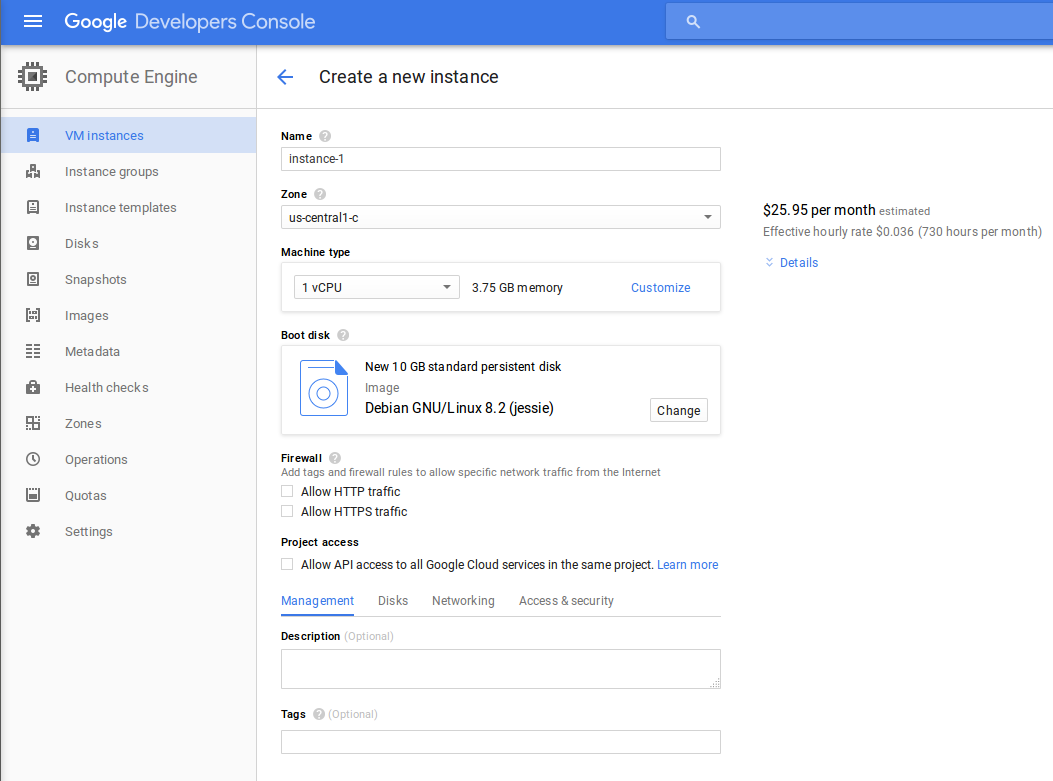
\includegraphics[scale=0.3]{figures/CreateInstance.png}
  \end{figure}
\end{frame}

\begin{frame}[fragile]
  \frametitle{Setting up instances}
  Things to choose at this point:
  \pause
  \begin{itemize}
  \item Number of cores, amount of RAM, size of disk, SSD or spinning
    \pause
  \item Operating system (Ubuntu, Centos, CoreOS), or choose a VM snapshot
    \pause
  \item Firewall rules
    \pause
  \item Whether to use static or ephemeral IP addresses (static IPs cost money!)
  \end{itemize}
\end{frame}

\begin{frame}[fragile]
  \frametitle{Setting up instances}
\end{frame}


\end{document}
